\section{Preliminaries: Data and User Models} 

In this section, we first describe our data model by reporting our data, visualization and query setup, and the underlying hierarchy of data subsets. We then discuss how analysts explore the hierarchy through a formative user study, and introduce our user model based on the findings of this study. Finally, we present our problem of finding an informative-and-interesting set of visualizations from the hierarchy.

%dor{added section on formative study, we need to put this somewhere} Our problem formulation is motivated by a formative study, where we asked participants to predict the value of a visualization after seeing a parent of the visualization to be predicted. In this between-group study, one group of participants were shown the informative parent, whereas another group of participants was shown the uninformative parents. Our main findings are : 1) it is natural for users to use the informative parent and 2) in the absence of informative parents, the users can be misled to have false expectations on the data.

\subsection{Data Model}
We start by discussing the data, visualization and query setup.

\textbf{Data.} We assume that we are operating on a dataset consisting of a single relational table $R$ with dimensions and measure attributes. Our approach also generalizes to multiple tables obeying a star or a snowflake schema, but we focus on the single table case for ease of presentation.

%\textbf{Visualization.} We define the notion of a visualization for our problem. There are different visualization types such as bar charts, scatter plots, and trend lines, but across all types, a visualization can be defined using five main components: (i) the x-axis attribute(s), (ii) the y-axis attribute, (iii) the subset of data used, (iv) the binning and aggregation functions for the x- and y- axes, and (v) the type of visualization (e.g., bar chart, scatter plot).

\textbf{Visualization.} We define the notion of a visualization for our problem. In our setup, a visualization can be defined using five main components: (i) the x-axis attributes, (ii) the y-axis attribute, (iii) the subset of data used (filter combination), (iv) the aggregation function for the y- axis, and (v) visualization type, e.g., bar chart.

\textbf{Query.} Our query setup applies to all visualization types that can be defined in terms of the aforementioned components, including common visualization types such as bar charts, trend lines, and scatter plots. Visualizations of these types can be translated into the following \textsc{SQL} query: {\tt SELECT X, A(Y) FROM R WHERE C(Z) GROUP BY X}. Here, $X$ refers to the x-axis attribute(s), $Y$ to the y-axis attribute, $A(Y)$ to the aggregation function on $Y$, $Z$ to the attribute(s) used in specifying the data subset, and $C(Z)$ to the constraints or filters that specify the data subset.\haz{we should discuss any limitations on the aggregation function here.}

Now, we discuss the set-theory based \emph{containment} relationships for data subsets, and based on the relationships introduce our hierarchy.

\textbf{Containment.} Given a data subset defined by a set of constraints $C = \{z_1, \ldots, z_n\}$, expanding $C$ by adding one or more new constraints will generate a new data subset that is contained within the former subset. An ancestor-descendant relationship exists between these data subsets. Specifically, a data subset defined by constraints $C_a$ is an ancestor of a data subset defined by constraints $C_b$, if and only if $C_b \subsetneqq C_a$. Further, a data subset defined by constraints $C_a$ is a parent of a data subset defined by constraints $C_b$, if and only if $C_b \subsetneqq C_a \land \mid C_a \mid - \mid C_b \mid = 1$. For example, given a dataset with three binary attributes {\tt \{P, Q, R\}}, the data subset defined by constraints {\tt \{P = 0,Q = 1\}} has two parents--- the data subset defined by constraint {\tt \{P = 0\}} and the data subset defined by constraint {\tt \{Q = 1\}}.

\textbf{Hierarchy.} Based on the containment relationship, we can organize the data subsets of a given dataset to form a hierarchy. This hierarchy of data subsets is overlaid on top of the lattice of attribute combinations. In data cube literature, the attribute combinations are called cuboids, and the data subsets are called cells. In Figure 1 we show the hierarchy of data subsets for a dataset with three binary attributes {\tt \{P, Q, R\}}, where we highlight the data subsets that belong to the same attribute combination with the same color. For example, all data subsets with three filters (at the lowest level of hierarchy) belong to the same attribute combination {\tt \{P, Q, R\}}, and are highlighted in dark gray. 

\begin{figure*}[ht!]
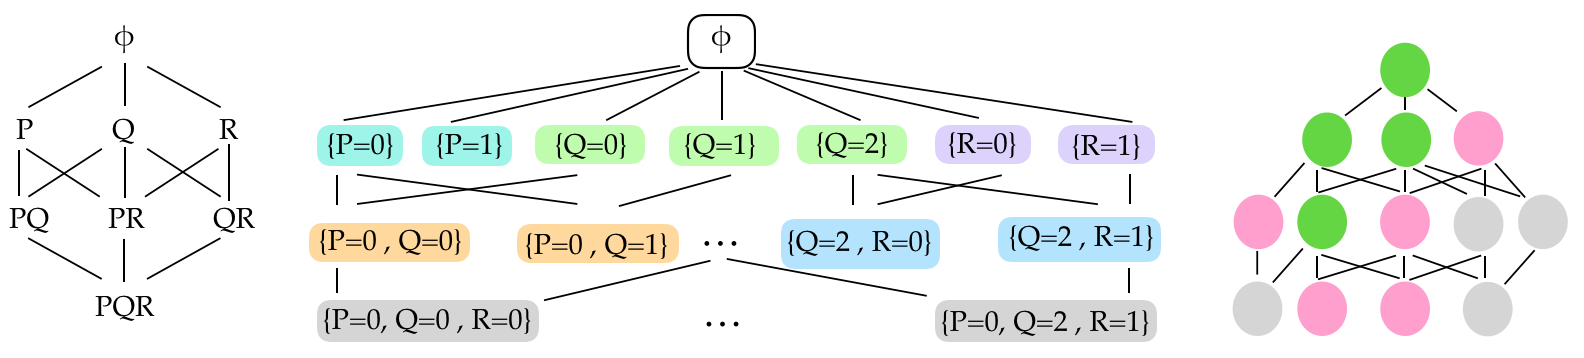
\includegraphics[width=\linewidth]{figures/lattice_frontier.pdf}
\caption{Left: Toy example demonstrating the notion of ``frontier''. Nodes that have been picked to include in the dashboard are colored green. The neighbors of the set of picked nodes are the frontier nodes, shown in pink. Grey nodes are other unpicked nodes in the lattice. Middle, Right: Hierarchy of data subsets for a dataset with three binary attributes {\tt \{P, Q, R\}}. The data subsets (called cells in datacubes) that belong to the same attribute combination (cuboid) are highlighted with same color.}
\label{fig:lattice}
\end{figure*}
\haz{Perhaps we can show another figure here (1a and 1b) of the lattice with the attributes only (no values) and same color scheme.}
We now extend the concept of \emph{containment} relationships (of data subsets) for visualizations defined according to our setup. 

\textbf{Viz Containment.} Let $V$ be the set of visualizations (of same type) that show the same $X$ and $Y$ for different $C(Z)$. Given a visualization $V_i \in V$, parent of $V_i$, $V_i^j$ ($V_i^j\in V$) is a visualization that corresponds to a parent data subset of the former. In Figure 2 we present three visualizations that show the survival rate of titanic passengers for three data subsets: (i) 3rd class passengers, (ii) female Passengers (3rd class and crew combined), (iii) 3rd class female passengers. As per the parent-child relationship among the data subsets, the visualizations corresponding to (i) and (ii) are parents of the visualization corresponding to (iii). %\hdev{Figure 2 example to be replaced with an example from Titanic. All three plots will be in the same row, with annotation (i), (ii), (iii).}

\begin{figure}[bht]
\label{example}
\centering
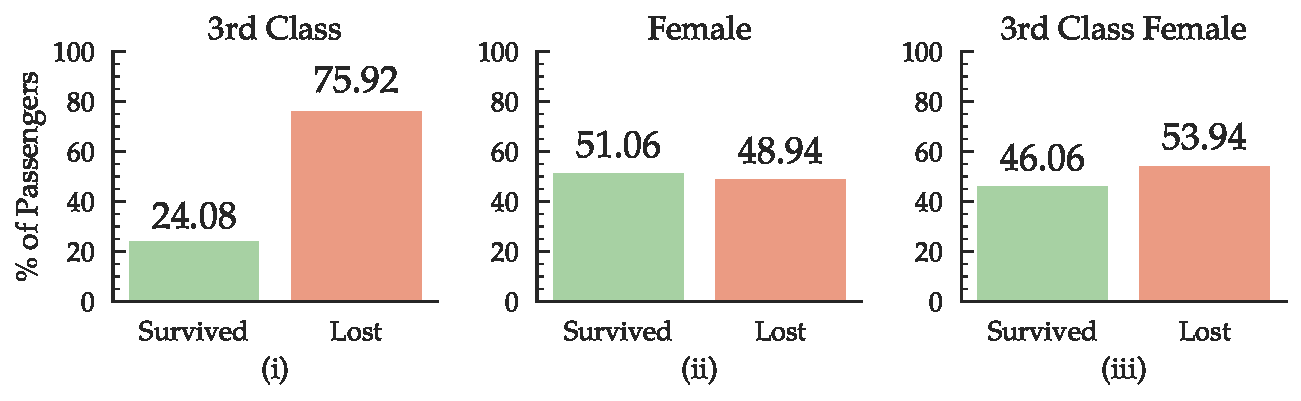
\includegraphics[scale=0.4]{figures/Titanic_Parent_Child.pdf}
\caption{Parent-child relationship amongst visualizations that show the survival rate of titanic passengers for three data subsets: (i) 3rd class passengers, (ii) female Passengers (3rd class and crew combined), (iii) 3rd class female passengers.}
\end{figure}\haz{Perhaps it will look better if have (iii) in a new line (and centered) to quickly reflect the parent-child relationship.}\dor{Considering that this will take up more space also not sure whether not sure we should mix up the problem formulation with the model itself. Himel?}

\textbf{Viz Hierarchy.} Based on the containment relationship of visualizations, we can organize the visualizations from $V$ to form a hierarchy. This hierarchy contains all visualizations (of same type, e.g., bar charts) that show the same x- and y- axes for different data subsets, and arranges them as per the parent-child relationships between data subsets. Our goal is to traverse this hierarchy of visualizations, and identify informative and interesting visualizations.

\subsection{User Expectation Model}
In order to identify which visualizations a user would deem informative and interesting, we first reveal how analysts explore the visualization hierarchy through a user study, and then model the effective utility of displaying an unseen visualization to a user in the context of other seen visualizations. 
 
\textbf{Top Down Traversal.} We observe that, while exploring a dataset, users first look at the top level visualizations before looking at the next level \cite{Kim2017, Hullman2013}. Further, the data distributions learnt from the top level visualizations induce user expectation for the next level. Based on these two observations, we model user expectation $\hat{V_i}$ corresponding to an unseen visualization $V_i$ based on its seen/observed parents $P(V_i) = \{V_i^1, \ldots, V_i^\lambda\}$ in the visualization hierarchy. 

\textbf{Formative User Study.} We conducted a user study to understand how a user's perception of an unseen visualization is affected by one or more of its observed parents. We recruited 9 participants to predict the distribution of an unseen visualization with two filters. Participants were asked to make a prediction regarding the unseen visualization after seeing the first parent displayed and subsequently after seeing the second parent displayed. In this between-group study, one group of participants (G1) were shown the first parent followed by the second parent, whereas another group of participants (G2) were shown the second parent followed by the first parent. Note that the two parent visualizations have different data distributions---the first parent well describes the unseen visualization, and the second parent differs from the unseen visualization. We examined how users form their expectation in presence of these observed parents. We summarize the results in Figure 2. Our main findings are : (1) it is natural for users to use one or more observed parents to form their expectation of an unseen visualization, (2) seeing an ``informative'' parent (that well describes the unseen visualization) leads to a better approximation of the unseen; (3) in absence of an informative parent, a user can be misled to form an inaccurate expectation; (4) in presence of multiple parents, the variance of expectation increases.
\dor{What about the surprisingness result? Should we discuss it here?}
\begin{figure}[bht]
\label{example}
\centering
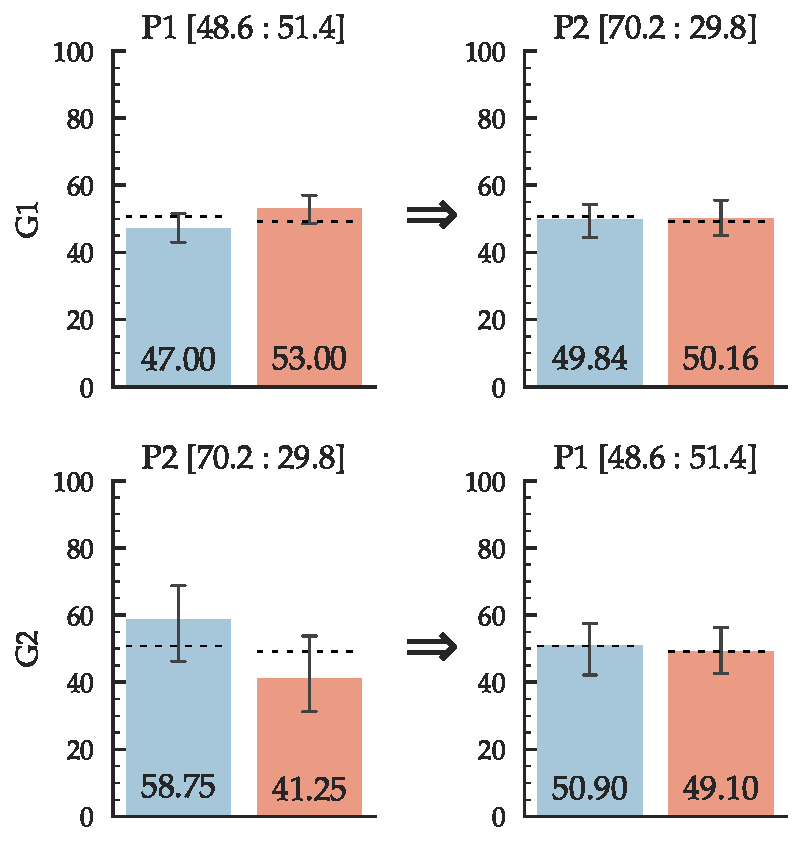
\includegraphics[scale=0.4]{figures/Formative_Study.pdf}
\caption{Results of the formative user study. The G1 participants were shown the informative parent first, followed by the uninformative parent; whereas G2 participants were shown the uninformative parent first, followed by the informative parent. The G1 participants closely approximated the unseen visualization immediately after seeing the informative parent.}
\end{figure}

Based on these findings, we model two aspects of the unseen-visualization and observed-parent relationship, namely informativeness and interestingness. 

\textbf{Informativeness.} To model the informativeness of an observed parent in the context of an unseen visualization, we characterize the capability of the parent in predicting the unseen visualization. For an unseen visualization, the observed parents whose data distributions well describe the data distribution of the unseen are \emph{informative}. Specifically, we formulate the informativeness of an observed parent $V_i^j$ ($V_i^j \in P(V_i)$) of an unseen visualization $V_i$ as the similarity between their data distributions using a similarity function $S(V_i, V_i^j)$. The most informative parents $V_i^*$ of an unseen visualization $V_i$ are the ones whose data distributions have highest similarity with that of the unseen.

\begin{equation}
    V_i^*=\underset{V_i^j}{argmax}\ S(V_i, V_i^j)
\end{equation}

Since declaring a parent as informative can vary depending on its similarity with the unseen compared to other parents, we allow the user to specify a threshold $\theta$, which we expect to be close to 1.0, such that the similarity score $S(V_i, V_i^{*, \theta})$ corresponding to the informative parents $V_i^{*, \theta}$ are at least $\theta\%$ of that of the most informative parents'. For example, if $\theta = 0.8$, all parents of $V_i$ whose similarity scores are at least 80\% of that compared to $V_i^*$ are deemed as informative. 

\begin{equation}
    V_i^{*, \theta} = \{V_i^j : \frac{S(V_i, V_i^j)}{S(V_i, V_i^*)} \ge \theta\}
\end{equation}

\textbf{Interestingness.} While the informative parents contribute to the prediction of an unseen visualization, the most interesting visualizations to recommend are those for which even the informative parents fail to predict the visualization. To model the interestingness of an unseen visualization $V_i$ in the context of an observed parent $V_i^j$ ($V_i^j \in P(V_i)$), we characterize the deviation between their data distributions using a distance function $D(V_i, V_i^j)$. The unseen visualizations whose data distributions deviate from the observed informative parents are \emph{interesting}. The most interesting unseen visualizations $V_\#$ are the ones that deviate most from their observed informative parents.
\begin{equation}
    V_\#=\underset{V_i}{argmax} \ D(V_i, V_i^{*, \theta})
\end{equation}

%\noindent Additional model extensions can be added to this objective function based user specification. For example, there may be $k$ visualizations that approximately yield equal contribution to the user's expectation. For simplicity of notation, we have assumed $k=1$ in the aforementioned model. In order, a user may want to prevent the recommendation of spuriously interesting subsets of the data. We can discard visualizations that falls below a certain subpopulation size threshold. 

\subsection{Problem Statement}

Given a dataset and user specified x- and y- axes, the goal of our system is to generate a dashboard by selecting $k$ visualizations from the hierarchy, where (1) one of the $k$ visualizations is the root--- the topmost visualization with no filters, (2) for each visualization except for the root, at least one of its informative parents is included within the $k$ visualizations, and (3) the $k$ visualizations are collectively most \lq\lq interesting\rq\rq\ in presence of their informative parents.

